\documentclass{article} % For LaTeX2e
\usepackage{nips13submit_e,times}
\usepackage{hyperref}
\usepackage{url}
\usepackage{verbatim}
\usepackage{graphicx}
\usepackage{subcaption}
\usepackage{listings}
%\documentstyle[nips13submit_09,times,art10]{article} % For LaTeX 2.09


\title{Incremental Construction of Programs in a Multitask Setting}

\begin{comment}
\author{
David S.~Hippocampus\thanks{ Use footnote for providing further information
about author (webpage, alternative address)---\emph{not} for acknowledging
funding agencies.} \\
Department of Computer Science\\
Cranberry-Lemon University\\
Pittsburgh, PA 15213 \\
\texttt{hippo@cs.cranberry-lemon.edu} \\
\And
Coauthor \\
Affiliation \\
Address \\
\texttt{email} \\
\AND
Coauthor \\
Affiliation \\
Address \\
\texttt{email} \\
\And
Coauthor \\
Affiliation \\
Address \\
\texttt{email} \\
\And
Coauthor \\
Affiliation \\
Address \\
\texttt{email} \\
(if needed)\\
}
\end{comment}
% The \author macro works with any number of authors. There are two commands
% used to separate the names and addresses of multiple authors: \And and \AND.
%
% Using \And between authors leaves it to \LaTeX{} to determine where to break
% the lines. Using \AND forces a linebreak at that point. So, if \LaTeX{}
% puts 3 of 4 authors names on the first line, and the last on the second
% line, try using \AND instead of \And before the third author name.

\newcommand{\fix}{\marginpar{FIX}}
\newcommand{\new}{\marginpar{NEW}}

%\nipsfinalcopy % Uncomment for camera-ready version

\begin{document}


\maketitle

\begin{abstract}
How can machine learning techniques be used to solve problems whose solutions are best represented as computer programs? For example, suppose a researcher wants to design a probabilistic graphical model for a novel domain. On the one hand, designing a good model requires a great deal of domain-specific knowledge and expertise, which may be hard to come by. On the other hand, searching the space of probabilistic models automatically is notoriously difficult. However, when researchers do set out to design graphical models, they draw on abstractions such as trees, chains, grids and plates to constrain and direct the kinds of models they produce. Thus, if we want to produce machine learning tools that aid in this task, we want tools that can learn these kinds of relevant abstractions. One natural way to think of these abstractions is as programs that take sets of random variables and produce graphical models that relate them. In this work, we describe the SEC algorithm, which attempts to learn distributions over such programs by incrementally finding program components that commonly help solve problems in a given domain. We discuss the behavior of the SEC algorithm for the task of graphical model structure learning. We also describe SEC's behavior on the dissimilar problem of automatically constructing tall and physically stable towers of blocks. 
\end{abstract}

\section{Introduction}


The vast majority of research in machine learning is focused on utilizing large amounts of noisy data living in high-dimensional, real-valued vector spaces. Such research has been immensely successful and has enabled automatic and accurate modelling on a scale that was previously infeasible. However, when we want to build a car, draw a painting, or design the machine learning models to which we apply our new algorithms and techniques, we face problems that current machine learning tools are unable to handle. The highly structured objects that humans produce seems to require a different representation than the ones which machine learning algorithms have most successfully employed. 

To address this problem, many structured representations have been proposed in the machine learning and AI literatures: learning over graphs \cite{}, grammars\cite{}, Horn clauses\cite{}, relations{}, etc., has been investigated. These are representations that attempt to bridge the gap between the tractablity of learning and reasoning in smooth continuous spaces and the expressivity of general purpose programming languages. 

However, many of the most natural representations of structured domains are best described as programs and are difficult to fit into more restrictive representations.  To take an example directly from the machine learning literature, consider the plate notation~\cite{DBLP:journals/jair/Buntine94} commonly used to describe graphical models over collections of variables. A typical example is shown in Figure~\ref{fig:lda_plate}~\cite{DBLP:journals/jmlr/BleiNJ03}. The goal of plate notation is precisely to express the notion of a ``for loop'' within the graphical model representation. One reason this is a convenient tool is that researchers conceptualize their models as sampling procedures -- easily expressed as programs (see Figure~\ref{fig:lda_code}, but not as static graphs -- and can use plate notation to express a commonly occuring control structure. In fact, the field of probabilistic programming, which has gained recent popularity, is spurred on by exactly the motivation that our models are most naturally expressed as programs. 

Suppose, then, that we want to create machine learning algorithms that can help discover good models for data in novel domains; that is, we want algorithms that discovers the structure of the latent graphical model underlying the data. This is a field of active research \ 

In this paper, we describe our approach to learning over structured representations as a search over the space of programs in a functional programming language. We characterize learning in this space as incrementally developing a weighted library of program abstractions, i.e. a collection of subroutines, that are commonly used to solve problems in a given domain. The SEC algorithm (for Sequential Exploration-Compression), which we present here, takes a set of related tasks and produces a distribution over programs that solve those tasks; as it refines this distribution, SEC is able to search the space of programs more efficiently and solve more tasks. 

We will present here two domains of interest. First, continuing with the example above, we will describe how SEC can learn to efficiently explore the space of relevant graphical models for a given problem. Second, we will examine SEC's performance on a completely different type of task, in which we want to an algorithm to build tall and physically stable block towers. 

\lstset{
	basicstyle=\scriptsize\ttfamily,
    commentstyle=\color{white!40!black},
    escapechar=+,
    escapebegin=\color{white!40!black},
    escapeend={},
    keywordstyle=\bfseries\color{Periwinkle},
    numbers=left,
    numberstyle=\sffamily\tiny\color{gray},
}


\begin{figure}[h]
\centering
\begin{subfigure}{.5\textwidth}
  \centering
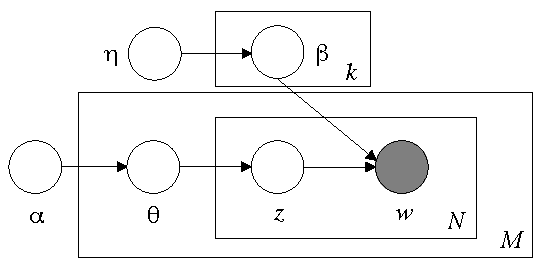
\includegraphics[width=.7\linewidth]{./figures/lda_plate_blei.pdf}
  \caption{An example of a typical plate notation use. \label{fig:lda_plate}}

\end{subfigure}%
\begin{subfigure}{.4\textwidth}
	\begin{lstlisting}[frame=single, numbers=none, xleftmargin=0pt]
	for +$k$+ = 1:NumTopics
	  +$\beta$+[k] +$\sim$+ Dirichlet(+$\eta$+)
	for m = 1:NumDocuments
	  +$\theta$+[m] +$\sim$+ Dirichlet(+$\alpha$+) 
	  for n = 1:NumWords 
	    z +$\sim$+ Categorical(+$\theta$+[m])
	    w+$\sim$+ Categorical(+$\beta$+[z])
	\end{lstlisting}
  \caption{The same model as a program.}
  \label{fig:lda_code}
\end{subfigure}
\caption{The popular Latent Dirichlet Allocation model in two forms.}
\label{fig:lda}
\end{figure}


\section{The SEC Algorithm}
\subsection{Generative Model}
Write down the generative model. Connect to EC and Percy Liang's work. Discuss ``programs as plans.''
\subsection{Inference}
Write down EM updates. Interpret them as a form of compression solved via a weighted Neville-Manning variant.

Discuss bootstrap learning: the right curriculum allows us to build more complicated programs.
Make some analogy involving how humans learn to paint, write poetry, bake, compose music, play with blocks, or design statistical models.

\subsection{Program Representation}
Discuss combinatory logic and the adaptor-grammar-esque distribution we use.

\section{Application to Structure Learning}
Learning the structure of graphical models is a difficult problem - not only for machines, but also for humans, where expert knowledge is often required.
In practice, the sorts of graphical models that humans design, such as Hidden Markov Models, phylogenetic trees, topic models, and Ising models, exhibit certain symmetries and recursive structures that are amenable to synthesis by programs.
Could an algorithm, such as SEC, automatically learn these structures?

\subsection{Graph Combinators}

Diagrams illustrating the graph combinators. An example program that makes an Ising model.

\subsection{Learning Graphical Models}

Show the actual results for our test cases: ``density estimation of the space of interesting graphical models.''
In future work, could be used as high-level moves in the search for a good structure.
Connect to, eg, Charles Kemp's work.

\section{Building Towers in Blocks World}

How could an agent, endowed with little prior knowledge, learn to build tall, robust towers out of toy blocks?
Although the space of possible towers is large enough to make exhaustive search intractible, the useful towers lie within a much smaller space.
Most useful towers use compositions of stereotyped structures, such as arches.

\subsection{The Blocks World Domain}

Tower representation, objective function

\subsection{Learned Tower programs}

Picture of tower. Grammar that produced that tower. Note lack of abstraction in grammar; speculate as to reasons.

\section{Discussion}

\subsection{Relation to Prior Work}

MH sampling of programs, ILP, Kitzelman, graph grammars

\subsection{Limitations of SEC}

Does not look at data. Does everything top-down. Blind to the utility of trying one program versus another (no active learning)

\section{Submission of papers to NIPS 2013}

NIPS requires electronic submissions.  The electronic submission site is  
\begin{center}
   \url{http://papers.nips.cc}
\end{center}

Please read carefully the
instructions below, and follow them faithfully.
\subsection{Style}

Papers to be submitted to NIPS 2013 must be prepared according to the
instructions presented here. Papers may be only up to eight pages long,
including figures. Since 2009 an additional ninth page \textit{containing only
cited references} is allowed. Papers that exceed nine pages will not be
reviewed, or in any other way considered for presentation at the conference.
%This is a strict upper bound. 

Please note that this year we have introduced automatic line number generation
into the style file (for \LaTeXe and Word versions). This is to help reviewers
refer to specific lines of the paper when they make their comments. Please do
NOT refer to these line numbers in your paper as they will be removed from the
style file for the final version of accepted papers.

The margins in 2013 are the same as since 2007, which allow for $\approx 15\%$
more words in the paper compared to earlier years. We are also again using 
double-blind reviewing. Both of these require the use of new style files.

Authors are required to use the NIPS \LaTeX{} style files obtainable at the
NIPS website as indicated below. Please make sure you use the current files and
not previous versions. Tweaking the style files may be grounds for rejection.

%% \subsection{Double-blind reviewing}

%% This year we are doing double-blind reviewing: the reviewers will not know 
%% who the authors of the paper are. For submission, the NIPS style file will 
%% automatically anonymize the author list at the beginning of the paper.

%% Please write your paper in such a way to preserve anonymity. Refer to
%% previous work by the author(s) in the third person, rather than first
%% person. Do not provide Web links to supporting material at an identifiable
%% web site.

%%\subsection{Electronic submission}
%%
%% \textbf{THE SUBMISSION DEADLINE IS MAY 31st, 2013. SUBMISSIONS MUST BE LOGGED BY
%% 23:00, MAY 31st, 2013, UNIVERSAL TIME}

%% You must enter your submission in the electronic submission form available at
%% the NIPS website listed above. You will be asked to enter paper title, name of
%% all authors, keyword(s), and data about the contact
%% author (name, full address, telephone, fax, and email). You will need to
%% upload an electronic (postscript or pdf) version of your paper.

%% You can upload more than one version of your paper, until the
%% submission deadline. We strongly recommended uploading your paper in
%% advance of the deadline, so you can avoid last-minute server congestion.
%%
%% Note that your submission is only valid if you get an e-mail
%% confirmation from the server. If you do not get such an e-mail, please
%% try uploading again. 


\subsection{Retrieval of style files}

The style files for NIPS and other conference information are available on the World Wide Web at
\begin{center}
   \url{http://www.nips.cc/}
\end{center}
The file \verb+nips2013.pdf+ contains these 
instructions and illustrates the
various formatting requirements your NIPS paper must satisfy. \LaTeX{}
users can choose between two style files:
\verb+nips11submit_09.sty+ (to be used with \LaTeX{} version 2.09) and
\verb+nips11submit_e.sty+ (to be used with \LaTeX{}2e). The file
\verb+nips2013.tex+ may be used as a ``shell'' for writing your paper. All you
have to do is replace the author, title, abstract, and text of the paper with
your own. The file
\verb+nips2013.rtf+ is provided as a shell for MS Word users.

The formatting instructions contained in these style files are summarized in
sections \ref{gen_inst}, \ref{headings}, and \ref{others} below.

%% \subsection{Keywords for paper submission}
%% Your NIPS paper can be submitted with any of the following keywords (more than one keyword is possible for each paper):

%% \begin{verbatim}
%% Bioinformatics
%% Biological Vision
%% Brain Imaging and Brain Computer Interfacing
%% Clustering
%% Cognitive Science
%% Control and Reinforcement Learning
%% Dimensionality Reduction and Manifolds
%% Feature Selection
%% Gaussian Processes
%% Graphical Models
%% Hardware Technologies
%% Kernels
%% Learning Theory
%% Machine Vision
%% Margins and Boosting
%% Neural Networks
%% Neuroscience
%% Other Algorithms and Architectures
%% Other Applications
%% Semi-supervised Learning
%% Speech and Signal Processing
%% Text and Language Applications

%% \end{verbatim}

\section{General formatting instructions}
\label{gen_inst}

The text must be confined within a rectangle 5.5~inches (33~picas) wide and
9~inches (54~picas) long. The left margin is 1.5~inch (9~picas).
Use 10~point type with a vertical spacing of 11~points. Times New Roman is the
preferred typeface throughout. Paragraphs are separated by 1/2~line space,
with no indentation.

Paper title is 17~point, initial caps/lower case, bold, centered between
2~horizontal rules. Top rule is 4~points thick and bottom rule is 1~point
thick. Allow 1/4~inch space above and below title to rules. All pages should
start at 1~inch (6~picas) from the top of the page.

%The version of the paper submitted for review should have ``Anonymous Author(s)'' as the author of the paper.

For the final version, authors' names are
set in boldface, and each name is centered above the corresponding
address. The lead author's name is to be listed first (left-most), and
the co-authors' names (if different address) are set to follow. If
there is only one co-author, list both author and co-author side by side.

Please pay special attention to the instructions in section \ref{others}
regarding figures, tables, acknowledgments, and references.

\section{Headings: first level}
\label{headings}

First level headings are lower case (except for first word and proper nouns),
flush left, bold and in point size 12. One line space before the first level
heading and 1/2~line space after the first level heading.

\subsection{Headings: second level}

Second level headings are lower case (except for first word and proper nouns),
flush left, bold and in point size 10. One line space before the second level
heading and 1/2~line space after the second level heading.

\subsubsection{Headings: third level}

Third level headings are lower case (except for first word and proper nouns),
flush left, bold and in point size 10. One line space before the third level
heading and 1/2~line space after the third level heading.

\section{Citations, figures, tables, references}
\label{others}

These instructions apply to everyone, regardless of the formatter being used.

\subsection{Citations within the text}

Citations within the text should be numbered consecutively. The corresponding
number is to appear enclosed in square brackets, such as [1] or [2]-[5]. The
corresponding references are to be listed in the same order at the end of the
paper, in the \textbf{References} section. (Note: the standard
\textsc{Bib\TeX} style \texttt{unsrt} produces this.) As to the format of the
references themselves, any style is acceptable as long as it is used
consistently.

As submission is double blind, refer to your own published work in the 
third person. That is, use ``In the previous work of Jones et al.\ [4]'',
not ``In our previous work [4]''. If you cite your other papers that
are not widely available (e.g.\ a journal paper under review), use
anonymous author names in the citation, e.g.\ an author of the
form ``A.\ Anonymous''. 


\subsection{Footnotes}

Indicate footnotes with a number\footnote{Sample of the first footnote} in the
text. Place the footnotes at the bottom of the page on which they appear.
Precede the footnote with a horizontal rule of 2~inches
(12~picas).\footnote{Sample of the second footnote}

\subsection{Figures}

All artwork must be neat, clean, and legible. Lines should be dark
enough for purposes of reproduction; art work should not be
hand-drawn. The figure number and caption always appear after the
figure. Place one line space before the figure caption, and one line
space after the figure. The figure caption is lower case (except for
first word and proper nouns); figures are numbered consecutively.

Make sure the figure caption does not get separated from the figure.
Leave sufficient space to avoid splitting the figure and figure caption.

You may use color figures. 
However, it is best for the
figure captions and the paper body to make sense if the paper is printed
either in black/white or in color.
\begin{figure}[h]
\begin{center}
%\framebox[4.0in]{$\;$}
\fbox{\rule[-.5cm]{0cm}{4cm} \rule[-.5cm]{4cm}{0cm}}
\end{center}
\caption{Sample figure caption.}
\end{figure}

\subsection{Tables}

All tables must be centered, neat, clean and legible. Do not use hand-drawn
tables. The table number and title always appear before the table. See
Table~\ref{sample-table}.

Place one line space before the table title, one line space after the table
title, and one line space after the table. The table title must be lower case
(except for first word and proper nouns); tables are numbered consecutively.

\begin{table}[t]
\caption{Sample table title}
\label{sample-table}
\begin{center}
\begin{tabular}{ll}
\multicolumn{1}{c}{\bf PART}  &\multicolumn{1}{c}{\bf DESCRIPTION}
\\ \hline \\
Dendrite         &Input terminal \\
Axon             &Output terminal \\
Soma             &Cell body (contains cell nucleus) \\
\end{tabular}
\end{center}
\end{table}

\section{Final instructions}
Do not change any aspects of the formatting parameters in the style files.
In particular, do not modify the width or length of the rectangle the text
should fit into, and do not change font sizes (except perhaps in the
\textbf{References} section; see below). Please note that pages should be
numbered.

\section{Preparing PostScript or PDF files}

Please prepare PostScript or PDF files with paper size ``US Letter'', and
not, for example, ``A4''. The -t
letter option on dvips will produce US Letter files.

Fonts were the main cause of problems in the past years. Your PDF file must
only contain Type 1 or Embedded TrueType fonts. Here are a few instructions
to achieve this.
=======
>>>>>>> 0c3d0be073ba9aaf201c99bcf3dc620f5bb9f7cb

\bibliographystyle{plain}
\bibliography{nips2013}

\end{document}
